\section{Evaluation}
\label{sec:Evaluation}
In this section we show different experiments that were run using the different parsers and analyse their running times, as well as the number of iterations in the inner most loop or their recursive calls respectively.
All configurations were parsed at least 10 times.
The time discussed in the following is the average running time of those runs, excluding the fastest and slowest run.
While the running time may vary for runs of the same configuration, the counter remains the same, as it is not influenced by external factors.

First, we give an overview over different grammars, that were used, and explain how we expect the algorithms to behave when parsing input strings on them.
All of them are in reduced Chomsky Normal Form, if not stated otherwise.

\subsection{Grammars}
\subsubsection{Dyck Language}
This language consists of all words, that have the correct amount of opening and closing parentheses, i.e., strings of the form \texttt{()...()}or \texttt{((...))}.
The grammar that builds these words has the productions:
\begin{align*}
    S&\rightarrow SS|LA|LR\\
    A&\rightarrow SR\\
    L&\rightarrow (\\
    R&\rightarrow )\\
\end{align*}

We ran experiments on words of the language, as well as on strings with additional single parentheses, i.e., \texttt{)()...()}and \texttt{()...()(}, which are not part of the language.

We expect top-down to run faster on strings of the form \texttt{()..()}.
The algorithm iterates over the productions in the order in which they were given to the program, thus $S\rightarrow SS$ is the first production.
It then iterates over different splitting points, starting with $k=1$, which will not find a solution, as $S$ can not yield any of the substrings, since they have a different amount of opening and closing parentheses.
When trying $k=2$, \texttt{Top-Down($S$, $1$, $2$)} is called, which returns \textit{true}.
For the right hand side of the string, this is repeated.
Thus, with the first production of the grammar and the second splitting point, the optimal answer is returned and the algorithm is expected to terminate relatively fast.

For strings of the form \texttt{((..))}, the top-down algorithm looks at a lot more subproblems while looking for the solution.
Opposed to strings of the form \texttt{()..()}, \texttt{((..))} has no partitioning into two substrings, where $S\rightarrow SS$ can yield both substrings.
In fact, all productions must be applied at least once for strings of this form to be produced.
Thus more productions and subproblems are considered before the answer is found.

Further, \texttt{)()..()}is parsed faster than \texttt{()..()(}by the top-down algorithm.
The way the algorithm was implemented, the right part of a splitting (second call of \texttt{Top-Down} on line~\ref{lst:td_call} in algorithm~\ref{alg:td}) will not be considered, if the left side returns \textit{false}.
This means, when the first symbol in the string violates the constraints of the language, the left-hand side of every partitioning can not be derived, and the right side will never be considered.
If, on the other hand, the last symbol violates the constraint, the algorithm finds for a lot of splitting points that $S$ can derive the left substring, and parses the right substring too.
This yields a lot more subproblems which have to be considered.
Thus, strings with an error in front are parsed faster than strings of the same form but with an error at the end


\paragraph{Linear Form}
\label{par:dyck_linear}
We will use this grammar to compare the non-specialized CYK algorithm to the algorithm adapted to grammars in linear form.
Therefore, the productions of the grammar are be transformed, such that the variables $L,R\in V$ can be omitted:
\begin{align*}
    S&\rightarrow (A\\
    A&\rightarrow )S|S)|)\\
\end{align*}

This is an equivalent grammar for the Dyck language.
When the parser transforms the grammar back to CNF, the resulting grammar has one non-terminal rule less than the initial grammar.
His is, since two more non-terminal variables (one for each parenthesis) are added, such that the transformed set of productions will be very similar to the initial grammar.
The parser is thus expected to yield slightly faster running times, if the linear grammar is transformed into CNF.
However, it might be faster, if this transformation is not performed, but the specialized algorithms are used.

\subsubsection{Strings Starting or Ending in a}
These grammars contain all worlds with an arbitrary number of \texttt{a}'s and \texttt{b}'s in any order, but starting resp. ending in a.
The productions for \textit{strings starting in a} are:
\begin{align*}
    S&\rightarrow AB\\
    B&\rightarrow BB|a|b\\
    A&\rightarrow a\\
\end{align*}

and those for \textit{strings ending in a}:
\begin{align*}
    S&\rightarrow BA\\
    B&\rightarrow BB|a|b\\
    A&\rightarrow a\\
\end{align*}

For both of these grammars we will run tests on strings of the form \texttt{ab..a} and \texttt{ba..ba}.
To analyse what running times are to be expected, we consider how $tab$ is filled by the algorithms.
$tab$ for this grammar is $3\times n\times n$, since it has three non-terminal variables.
We look at the two dimensional table of each non-terminal in turn.

The table for $A$, say $tab_A$, has \textit{true} only in the row for substrings of length 1 and where the symbol is \texttt{a}.
As it has no non-terminal production, when trying to fill the reminder of $tab_A$ the algorithm proceeds very fast.

The table for $B$, $tab_B$, has \textit{true} in all cells.
All substrings of length one can be derived, since $B$ has the two terminal productions $B\rightarrow a|b$.
Further, since its only non-terminal production is $B\rightarrow BB$, when trying to fill a new cell of $tab_B$, only other cells of $tab_B$ must be considered.
Because they are all \textit{true}, the loop over $k$ is braked after trying the first splitting point and the cell is set to \textit{true}.
Thus filling $tab_B$ can be done in a fast matter, too.

We now look at $tab_S$.
For \textit{strings starting in a} the only production for $S$ is $S\rightarrow AB$, thus the cell of $tab_A$ is accessed first.
The first splitting point always generates a substring of length one, on the left of $k$.
If this is an \texttt{a}, then the corresponding cell in $tab_A$ is \textit{true}, and we must access $tab_B$ as well.
As we argued before, this value will always be \textit{true}, we are thus not looking at any other splitting points.
If the first symbol of the substring is \texttt{b}, then the cell in $tab_A$ is \textit{false}, and we will not look at $tab_B$, but continue to the next splitting point.
This will be repeated for all further $k$, because $tab_A$ is false for all substrings with length more than one.
Thus, the more \texttt{b}'s the input string has, the bigger the running time will be, since for all substrings starting with a \texttt{b}, all possible $k$ are considered.

For the grammar \textit{ending in a} the production for $S$ is $S\rightarrow BA$, thus for every splitting point first $tab_B$ gets accessed, which will always return \textit{true}.
Then $tab_A$ gets accessed, which will return \textit{false} in all cases, where the right substring is not \texttt{a}.
This implies, that all $k$ must be considered, since only for the last $k$, where the right substring has length one, $tab_A$ may be true.
Thus, all $k$ are considered for all substrings, whereas for \textit{starting in a} the loop gets braked after the first $k$, if the substring can be derived.
Further, both $tab_B$ and $tab_A$ are accessed for every $k$, while for \textit{starting in a} $tab_B$ was only accessed when $tab_A$ was \textit{true}.

In conclusion, \textit{ending in a} may perform more than twice the amount of table accesses than \textit{starting in a}, and its running time is higher.
We further expect bottom-up to have very similar running times on any input string of the same length for \textit{ending in a}, while the times for \textit{starting in a} depend on the amount of \texttt{b}'s in the substring.
Top-down is expected to behave very similar, but will be faster on \textit{starting in a} than bottom-up, since it looks at less subproblems.

\todo{read this part again, since restructured a lot}


% \subsubsection{Equal Numbers}
% Equal numbers is a grammar, that yields all strings with the same amount of a's and b's.
% This is achieved with the following productions:
% \begin{align*}
%     S&\rightarrow SS|AB|BA\\
%     B&\rightarrow SB|BS|b\\
%     A&\rightarrow a\\
% \end{align*}

% For this grammar we test strings of the form \texttt{ aa..bb}and \texttt{ ab..ab}, as well as both of these sets with additional a's.
% We expect the parsers to yield similar running times on this grammar and for this input strings, than parsing \texttt{()...()}and \texttt{((...))} respectively for the Dyck language
% since the arrangement of the terminal symbols is very similar, with a and b instead of opening and closing parentheses.
% The cases that should return \textit{false} are probably slower, since this grammar has one production more than the grammar for the \textit{Dyck language}.

\subsubsection{ABC Grammar}
The language of this grammar is more complicated to explain than the grammars before.
The simplest grammar describing it is $G=(\{S\}, \{a,b,c\},P,S)$, where $P$ is:
\begin{align*}
    S&\rightarrow aSc|abSc|b\\
\end{align*}
The words in the corresponding language $L(G)$ can be divided into three parts:
\begin{itemize}
    \item The first part starts with an \texttt{a}, and  consists of \texttt{a} 's and \texttt{b} 's, such that the number of \texttt{a} 's is equal or bigger to the number of \texttt{b} 's. There are never two \texttt{b} 's after each other without an \texttt{a}in between.
    \item In between the two parts is a \texttt{b} (this \texttt{b}may follow right after a \texttt{b}of the first part).
    \item The third part consists only of \texttt{c} 's, the number of \texttt{c} 's is equal to the number of \texttt{a} 's in the first part.
\end{itemize}

We will use this grammar only to evaluate the specialization, therefore we transform it to the equivalent linear grammar $G=(\{A,B,S\}, \{a,b,c\}, P, S)$ with the productions:
\begin{align*}
    S&\rightarrow Ac|b\\
    A&\rightarrow aS|aB\\
    B&\rightarrow bS\\
\end{align*}

The strings we will test are of the form \texttt{abab..b..cc}, \texttt{aa..b..cc} and the same with an additional \texttt{a} and \texttt{c} in the front or end respectively.


\subsection{Evaluation of the conventional Implementation}
We now show the results of experiments, using the grammars described, and analyze whether the algorithms behave as we expect them to behave.
For these tests, the conventional algorithms as described in sections \ref{sec:top_down}~and \ref{sec:bottom_up}~where used.

\subsubsection{Dyck Language}
\label{sec:eval_dyck}

\begin{figure}[!ht]
    \centering
    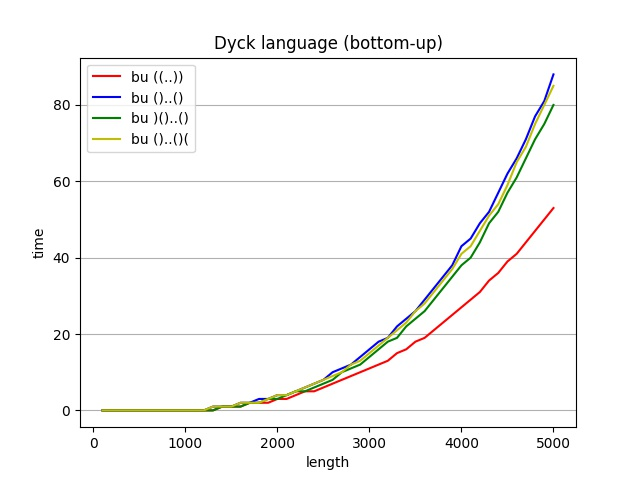
\includegraphics[width=0.6\textwidth]{Resources/t_dyck_bu.jpg}
    \caption{Running time (s) of the bottom-up algorithm when parsing different set of strings of sizes 100-5000, in steps of hundred, for the \textit{Dyck language}.}
    \label{fig:t_dyck_bu}
\end{figure}

Figure~\ref{fig:t_dyck_bu} shows the running times of the bottom-up parser on different sets of input strings for the grammar \textit{Dyck language}.
The strings were of length 100 to 5000, growing in steps of 100.
As expected, the times are very similar for three of the four different sets of input strings.
However, parsing the strings of the form \texttt{\texttt{((..))}}is a little faster.
When looking at how the $tab$ is filled, we see that $tab[A]$ is very similar in both cases.
$tab[S]$ on the other hand has \textit{true} in more cells for strings of the form \texttt{()..()} than \texttt{((..))}.
As we argued before, the loop over $k$ gets breaked, when both subproblems are true, which makes the parser more efficient.
Thus, more \textit{true} entries intuitively lead to faster running times, as the loop is executed less often.
For strings of the form \texttt{()..()}, this is not the case.
The additional \textit[true] in $tab[s]$ lead to a lot more table accesses, when the rule $S\rightarrow SS$ is considered.
Therefore strings of the form \texttt{\texttt{((..))}} can be parsed faster by the bottom-up algorithm.

The curves are asymptotically to $O(n^3)$, in fact, the yellow, blue and green line are very close to $6.4*10^{-10}*n^3$.

We split the parsings of top-down into two plots.
The first one, Figure~\ref{fig:t_dyck_td_slow}, is for the slow cases, where we did not run the parser on strings longer than 2500
The second one, Figure~\ref{fig:t_dyck_td_fast}, was for the fast cases, where we extended the test set to contain strings up to a size of 10000.

\begin{figure}[!ht]
    \centering
    \begin{subfigure}[b]{0.48\textwidth}
        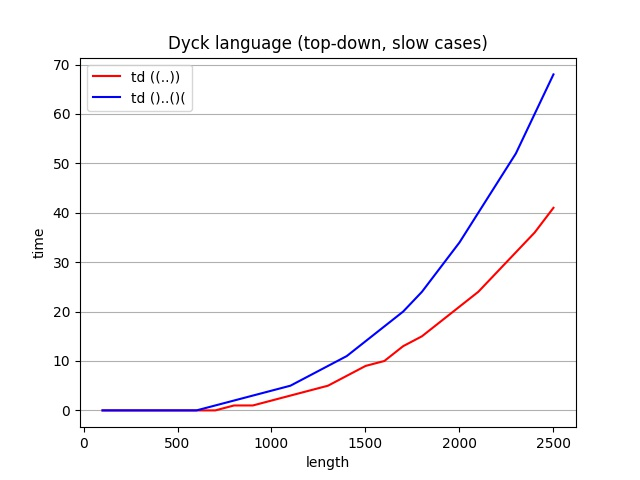
\includegraphics[width=1.1\textwidth]{Resources/t_dyck_td_slow.jpg}
        \caption{}
        \label{fig:t_dyck_td_slow}
    \end{subfigure}
    \hfill
    \begin{subfigure}[b]{0.48\textwidth}
        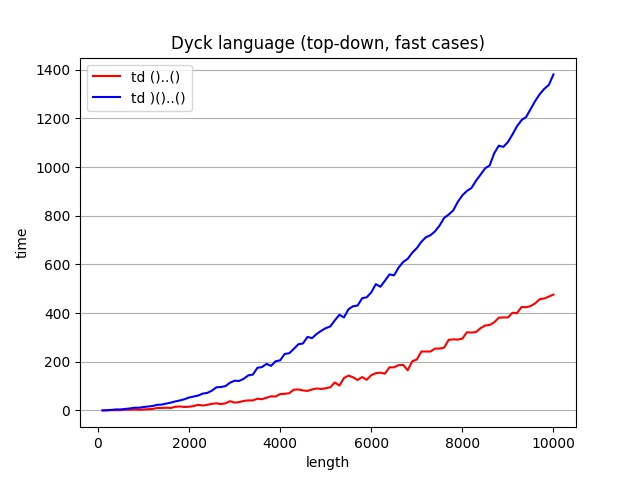
\includegraphics[width=1.1\textwidth]{Resources/t_dyck_td_fast.jpg}
    \caption{R}
    \label{fig:t_dyck_td_fast}
    \end{subfigure}
    \caption{Running times in (a) seconds and (b) milliseconds for the top-down algorithm when parsing four sets of strings of sizes (a) 100-2500 and (b) 100-1000, in steps of hundred, for the \textit{Dyck language}.}
\end{figure}

As we assumed, parsing the test sets of strings of the form \texttt{((..))}and \texttt{()..()(}with top-down was a lot slower than parsing the strings of the other two sets.
While parsing strings of the form \texttt{()..()(}of length 2500 took almost 70 seconds, parsing strings of the form \texttt{()..()}of length 10'000 took only 0.4 seconds.

The fast cases are a lot faster than the bottom-up parser.
This is the case, because bottom-up fills all cells of $tab$, regardless of whether or not they are needed to find the solution, while top-down only fills the one needed to find the optimal solution.
When the productions of the grammar are in a favorable order and the splitting points for finding subproblems that yield the optimal solution is low, as it is the case in the fast cases of Dyck, it can be very fast.

However, if this is not the case, then the parser may take a lot of time.
We can see this at the slow cases of the \textit{Dyck language}.
Here, the parser behaves a lot worse than bottom-up.
This may be due to the fact, that bottom-up fills the cells of $tab$ in a structured way, accessing the already filled cells of $tab$ not more often, then needed to fill the other cells.
Top-down on the other hand may run into the same subproblems very often.
This means the algorithm calls itself recursively in order to access the cell of the same subproblem more often than bottom-up does.
Since recursive calls are more time consuming, and more accesses may be performed, this results in a potentially very bad running time.

\begin{figure}[!ht]
    \centering
    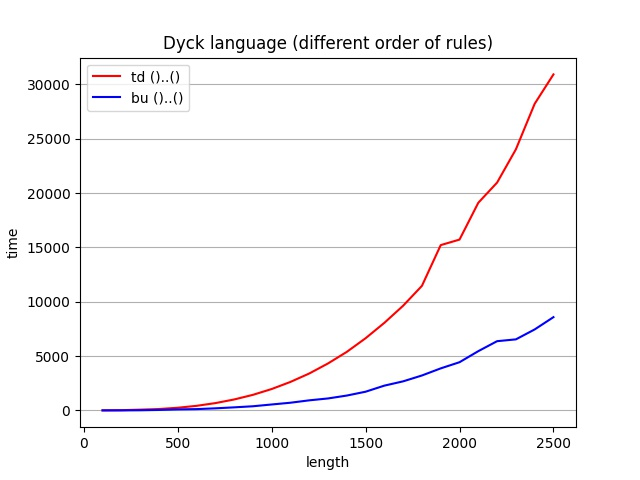
\includegraphics[width=0.6\textwidth]{Resources/t_dyck_order.jpg}
    \caption{Running time (ms) of both algorithms for parsing a set of strings of sizes 100-2500, in steps of hundred, for the \textit{Dyck language}, with a different order of the productions.}
    \label{fig:t_dyck_order}
\end{figure}

I order to verify the hypothesis, that the order of productions matters for the top-down parser, we run experiments on the same grammar, but with the productions of $S$ in opposite order.
The results can be seen in figure~\ref{fig:t_dyck_order}.
The parser is in fact a lot slower than it was before, thus the order of the productions may play a major role, when parsing.
The plot further shows that the order does not matter that much for the bottom-up parser.
It has almost the same running time, than it had with the original ordering of the productions.

\subsubsection{Strings starting and ending in a}

As expected, both the top-down and bottom-up algorithm performed very differently on the two grammars, being rather fast at parsing for the grammar \textit{starting in a}, and slower for \textit{ending in a}.
In general, we see that the times are lower than they were for the \textit{Dyck language}.
This is presumably because this grammar has only two non-terminal productions, which leads to less subproblems which have to be considered.

We split the results in three graphs; one for the running times of both parsers on the grammar \textit{ending in a} (Figure~\ref{fig:t_ea_td_bu}), one for top-down and one for bottom-up, each for the grammar \textit{starting in a} (Figures~\ref{fig:t_sa_td} and~\ref{fig:t_sa_bu} respectively).

\begin{figure}[!ht]
    \centering
    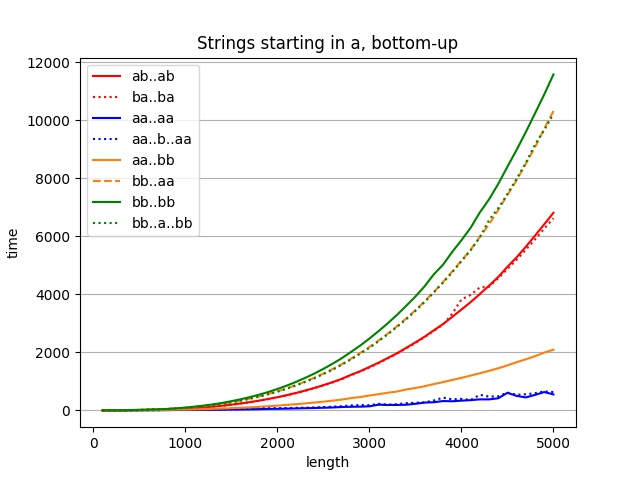
\includegraphics[width=0.6\textwidth]{Resources/t_sa_bu.jpg}
    \caption{Running time (ms) of the bottom-up algorithm when parsing sets of strings of sizes 100-2500, in steps of hundred, for the language of words starting in a.}
    \label{fig:t_sa_bu}
\end{figure}

Figure~\ref{fig:t_sa_bu} shows, that the running times of bottom-up indeed depends on the amount of \texttt{b}'s in the input string.
We see, that strings of the form \texttt{bb..bb} have the slowest running times, while strings of the form \texttt{aa..aa} are parsed very fast.
While adding an \texttt{a} to the first type does influence the running time, adding a single \texttt{b} to the second one has almost no influence.
Further, for strings with alternating letters (the red lines) the running time does not change if the string starts with \texttt{a} or \texttt{b}.
However, if the \texttt{a}'s and \texttt{b}'s are continuously (yellow lines), the strings are parsed a lot faster if the \texttt{a}'s are first.
\todo{add further analysy/reasoning?}

\begin{figure}[!ht]
    \centering
    \begin{subfigure}[b]{0.48\textwidth}
        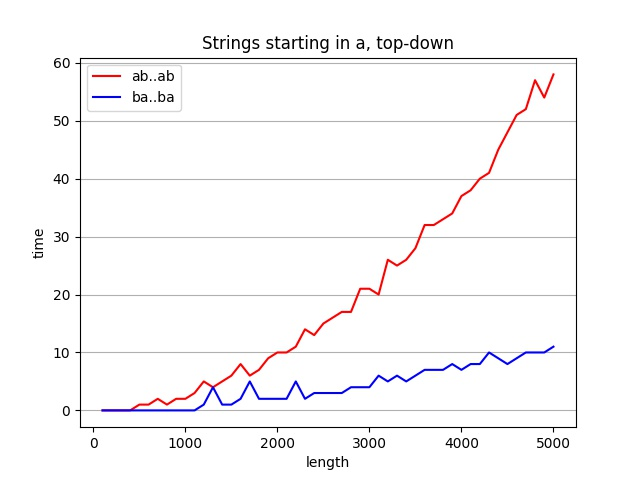
\includegraphics[width=1.1\textwidth]{Resources/t_sa_td.jpg}
        \caption{}
        \label{fig:t_sa_td}
    \end{subfigure}
    \hfill
    \begin{subfigure}[b]{0.48\textwidth}
        \centering
        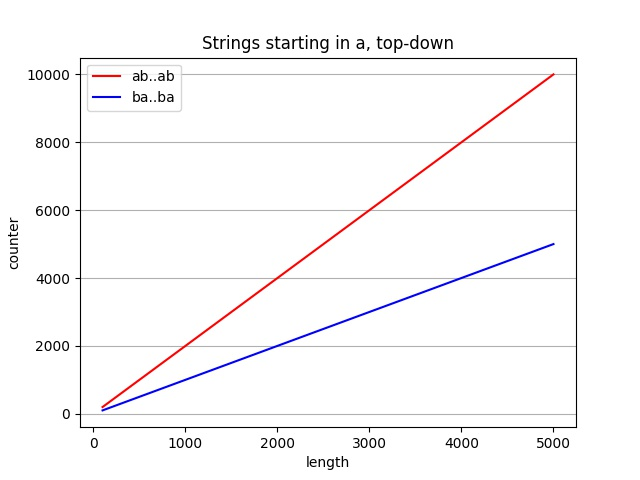
\includegraphics[width=1.1\textwidth]{Resources/c_sa_td.jpg}
        \caption{}
        \label{fig:c_sa_td}
    \end{subfigure}
    \caption{Sunning time in ms (a) and counter (b) of the top-down algorithm when parsing sets of strings of sizes 100-5000, in steps of hundred, for the Language of words starting in a.}
\end{figure}

Figure~\ref{fig:t_sa_td} shows the incredibly low running times of top-down on the grammar \textit{strings starting in a}.
The times are so low, since the algorithm does not fill $tab$ completely.
In fact, when parsing strings not starting in \texttt{a}for the grammar \textit{starting in a}, it will only ever look at the most left children of the recursive tree, since each of them returns \textit{false}.
This results in a very low amount of recursive calls as can be seen in figure~\ref{fig:c_sa_td}.
The number of calls on the recursive function is $\Theta(n)$ for parsing strings not starting in a for the grammar \textit{starting in a}.
As we argued in section~\ref{sec:top_down}, the upper bound for this number is $O(n^3)$.
The numbers for the counter of bottom-up (repetitions of the inner most loop, i.e. over splitting points $k$) for parsing strings for \textit{starting in a}, are somewhere in between of $n^2$ and $n^3$, still yielding relatively fast running times.

The three bumps in the running time of top-down on strings of the form \texttt{ba..ba}are supposedly due to rounding errors of the compiler, seen as the times there are lower than 5 milliseconds.
The bumps appear on the red line at the same time after the same period of time after starting the parsers (not at the same length of strings!), though not as distinctive as in the blue line, since the running times are already a little higher at this point.
The bumps could be reduced by running the parser 40 times per input string instead of 10 times which supports this theory.

\begin{figure}[!ht]
    \centering
    \begin{subfigure}[b]{0.48\textwidth}
        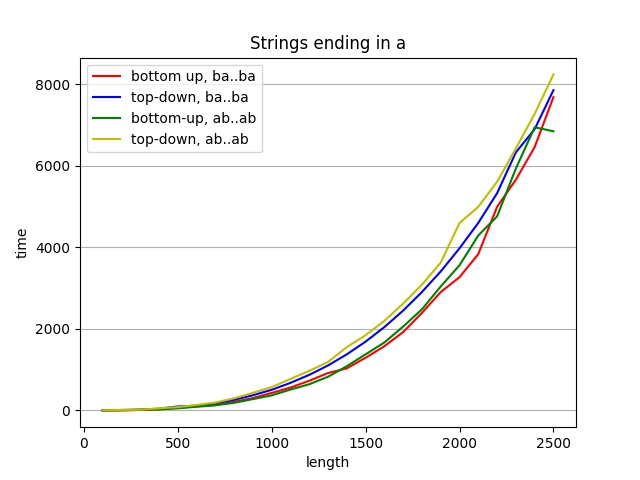
\includegraphics[width=1.1\textwidth]{Resources/t_ea_td_bu.jpg}
        \caption{}
        \label{fig:t_ea_td_bu}
    \end{subfigure}
    \hfill
    \begin{subfigure}[b]{0.48\textwidth}
        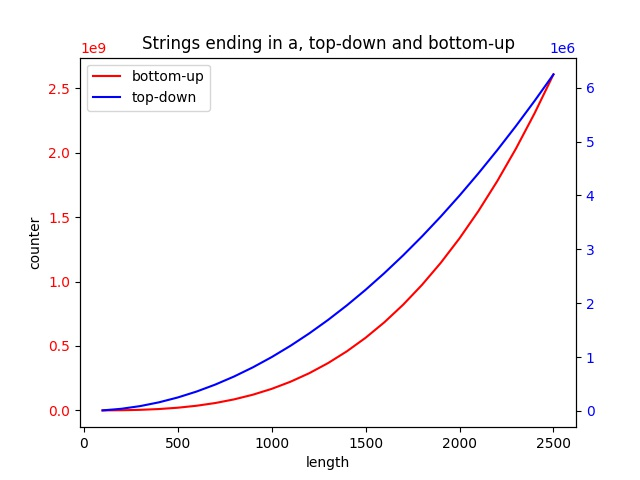
\includegraphics[width=1.1\textwidth]{Resources/c_ea_td_bu.jpg}
        \caption{}
        \label{fig:c_ea_td_bu}
    \end{subfigure}
    \caption{Running time in ms (a) and counter (b) of the bottom-up and top-down algorithm when parsing sets of strings of sizes 100-2500, in steps of hundred, for the language of words ending in a.}
\end{figure}

Figures~\ref{fig:t_ea_td_bu} and \ref{fig:c_ea_td_bu} show, that the curves for parsing the grammar \textit{ending in a} are almost identical with the ones of the bottom-up parser run on the \textit{Dyck language}.
We further see, that all of them have a very similar shape.
In fact, both the bottom-up and the top-down parser have the same counter respectively for any string of the same length, regardless of the order of the letters.
As can be seen in figure\ref{fig:c_ea_td_bu}, for a string of length 100, bottom-up iterates 171600 times of its most inner loop while top-down calls itself recursively 9901 times.
Despite this big difference of \texttt{counter}, the running times are almost identical for both algorithms.
This is due to the more efficient manner of bottom-up.
One aspect is the more structured way to allocate the cells of $tab$, the second one the fact that Java can not perform recursive functions as efficient as iterative ones. \todo{is here a citation needed?}


\subsection{Evaluation of the Specialization with Linear Grammars}
In order to test the specialization for linear grammars, we parse strings by using the grammar parser, which transforms the linear grammar provided to CNF.
Further, we compare the running times of parsing strings with the transformed grammar to parsing them with the specialized bottom-up algorithm.

\subsubsection{Grammar Transformation}
In order to test how parsing the grammar from a linear grammar to on in CNF, we use the linear form of the \textit{Dyck language} as introduced in \ref{par:dyck_linear}.
The comparison of those results to the results fo the evaluation of the initial \textit{Dyck Language} can be seen in figure~\ref{fig:t_c_dyck_lin_cnf}.
As expected, strings could be parsed slightly faster for the transformed grammar than for the initial form.
The plot further shows, that the linear bottom-up algorithm is a lot faster than the CNF one, and that the counter is perfectly asymptotical to the running time.

\begin{figure}[!ht]
    \centering
    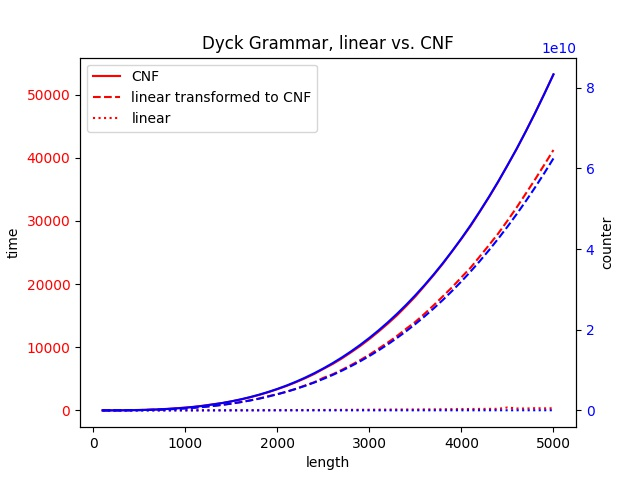
\includegraphics[width=0.6\textwidth]{Resources/t_c_dyck_lin_cnf.jpg}
    \caption{Running time (ms) and counter of the bottom-up algorithm when parsing strings of the form \texttt{((..))} for the Dyck language. \textit{CNF} is the running time of parsing with the productions of the initial grammar, \textit{linear transformed to cnf} the one for the linear productions, but transformed to CNF by the parser, and \textit{linear} the running times when the specialized CYK algorithm was used.}
    \label{fig:t_c_dyck_lin_cnf}
\end{figure}

The CNF-configuration refers to the bottom-up parser run on the initial grammar, time and counter are the same as in \ref{sec:eval_dyck}.
The second configuration used the linear transformation of the \textit{Dyck language}, but transformed it to CNF before parsing the strings.
This results in one non-terminal rule less, which is why the parser is slightly faster.
The third configuration parses strings for the linear grammar using the specialized algorithm.
It is a lot faster then both of the other configurations.
To analyse the difference between the linear and CNF parser better, we consult the experiments run on the \textit{abc grammar}.


\subsubsection{Adapted algorithm}
\begin{figure}[!ht]
    \centering
    \begin{subfigure}[b]{0.48\textwidth}
        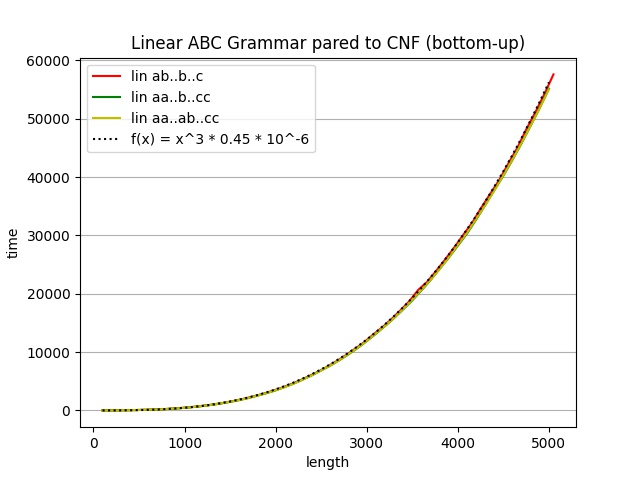
\includegraphics[width=1.1\textwidth]{Resources/t_abc_cnf.jpg}
        \caption{}
        \label{fig:t_abc_cnf}
    \end{subfigure}
    \hfill
    \begin{subfigure}[b]{0.48\textwidth}
        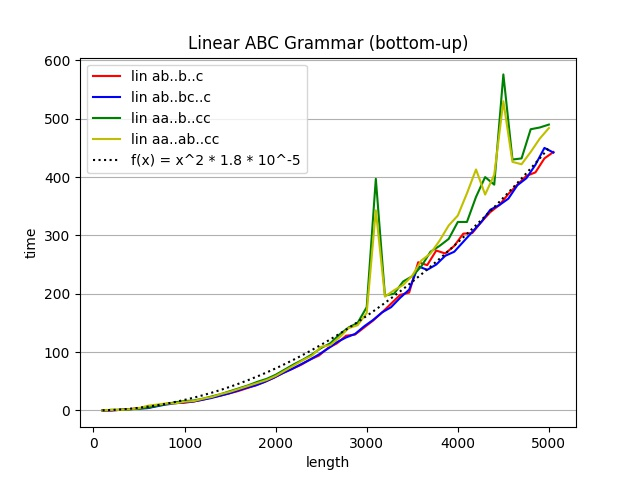
\includegraphics[width=1.1\textwidth]{Resources/t_abc_lin.jpg}
        \caption{}
        \label{fig:t_abc_lin}
    \end{subfigure}
    \caption{Running time in ms of the bottom-up algorithm when parsing strings for a linear grammar (a) by transforming the grammar to CNF and (b) by using the specialized algorithm. Both plots contain a function of the length as reference.}
\end{figure}

Figure \ref{fig:t_abc_cnf} shows the running time which is yielded when parsing strings for the \textit{abc grammar} by transforming the productions to CNF.
Since we used the bottom-up parser we expected the times to be very similar for all sets of input strings, which is the case.
The graph also contains a function over the length of the input strings, $f(x)=x^3*0.45*10^-6$, which shows that the running time indeed is in $O(n^3)$.
The specialized algorithm could parse the strings in a tenth of the time, the cnf parser needed.
This is partly due to the smaller amount of rules, but also because only one splitting point per rule has to be considered.
Here, the running times are very similar for all types of input strings, too.
The variations between the different types can be seen better, as the numbers are a lot smaller.
Like in Figure~\ref{fig:t_dyck_td_fast}, some configurations have bumps.
We explain them with the same reasoning, assuming they appear only because the algorithm is very fast.
The graph, too, contains a function over the length of the input strings, $f(x)=x^2*1.8*10^-5$,showing that the running time is in $O(n^2)$, as expected.
